\chapter{Wykład 13. Zarządzanie komunikacją w projekcie informatycznym}

\section{Interesariusze projektu}
% strona 29

\begin{enumerate}
	\item Interesariusz: Średnie przedsiębiorstwo realizujące projekt w oparciu o PMBOK
\begin{itemize}

	\item Pozycja: klient
	\item Rola: odbiorca produktu
	\item Wymagania: sprawne, niezawodne, łatwe w użytkowaniu oprogramowanie
	\item Oczekiwania: usprawni realizację projektu
	\item Wpływ/zainteresowanie: niski/wysokie
	\end{itemize}

	\item Interesariusz: Zespół projektowy firmy
\begin{itemize}

	\item Pozycja: zespół projektowy
	\item Rola: tworzenie produktu
	\item Wymagania: wynagrodzenie za swoją pracę
	\item Oczekiwania: dotrzymywanie terminów
	\item Wpływ/zainteresowanie: wysoki/średnie
	\end{itemize}

	\item Interesariusz: Inna firma z branży
\begin{itemize}

	\item Pozycja: konkurencja
	\item Rola: tworzenie oprogramowania
	\item Wymagania: przejęcie rynku
	\item Oczekiwania: fiasko naszego projektu
	\item Wpływ/zainteresowanie: niski/średnie
	\end{itemize}

	\item Interesariusz: Rada nadzorcza
\begin{itemize}

	\item Pozycja: zarząd
	\item Rola: nadzorowanie realizacji projektu firmy
	\item Wymagania: terminowość, powstanie finalnego produktu
	\item Oczekiwania: wysoki zysk, wysoka jakość
	\item Wpływ/zainteresowanie: niski/wysokie
	\end{itemize}

	\item Interesariusz: Marketing
\begin{itemize}

	\item Pozycja: dział przedsiębiorstwa
	\item Rola: rozreklamowanie produktu
	\item Wymagania: terminowość
	\item Oczekiwania: popyt
	\item Wpływ/zainteresowanie: niski/niskie
	\end{itemize}

	\item Interesariusz: TVN
\begin{itemize}

	\item Pozycja: media
	\item Rola: reklama produktu
	\item Wymagania: spot zgodny z regulaminem
	\item Oczekiwania: wysoka oglądalność reklamy
	\item Wpływ/zainteresowanie: średni/niskie
	\end{itemize}

\end{enumerate}

\clearpage

% ===========================================================================

\section{Plan przekazywania informacji}
% strona 40

Przekazywanie informacji w projekcie: 

\begin{figure}[!h]
\centering
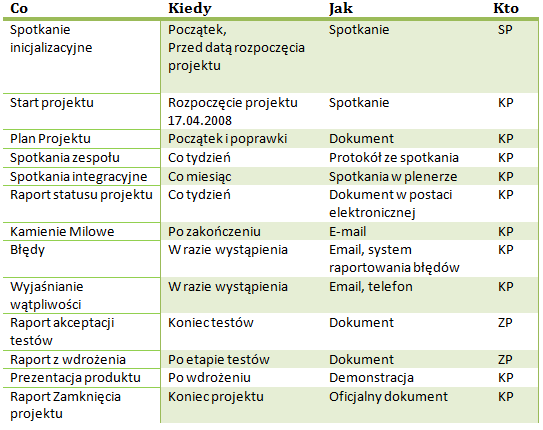
\includegraphics[width=\textwidth]{przekazywanieInformacji.png}
\caption{Plan przekazywania informacji}
\label{fig:przekazywanieInformacji}
\end{figure}

%\clearpage

Przekazywanie innym osobom informacji o projekcie:
 Do przekazywania informacji o projekcie (udziałowcom lub osobom, którym przydzielono pracę) można skorzystać z takich funkcji jak:
\begin{itemize}
\item Drukowanie i raportowanie, aby przedstawić innym informacje o projekcie na papierze. 
\item Publikowanie w formacie HTML lub zapisywanie planu projektu na serwerze sieci Web, aby dać innym dostęp do informacji o projekcie w witrynie sieci Web. 
\item Program Microsoft Project Central lub grupy robocze, aby używać programu Microsoft Project Central zainstalowanego w firmowej sieci intranet lub w Internecie albo systemu poczty e-mail w celu przekazywania innym informacji o projekcie. 
\item Integracja z programem Microsoft Outlook, aby inne osoby przeglądały zadania na swoich listach zadań programu Outlook.
\end{itemize}


% ===========================================================================

\section{Szablon spotkania i notatki ze spotkania}

% strona 65

Spotkania odbywają się według ściśle określonego harmonogramu:
\begin{enumerate}
	\item Przegląd stanu realizacji założeń poprzedniego spotkania.
	\item Przegląd rozwiązań powstałych poprzednio problemów.
	\item Omówienie celi do zrealizowania przed kolejnym spotkaniem.
	\item Podział zadań
	\item Identyfikacja nowych problemów, powstałych od poprzedniego spotkania.
	\item Dyskusja na temat rozwiązania zidentyfikowanych problemów.
	\item Uwagi dotyczące sposobu realizacji projektu.
\end{enumerate}

\clearpage

\subsection*{Szablon notatki ze spotkania}

\begin{figure}[!h]
\centering
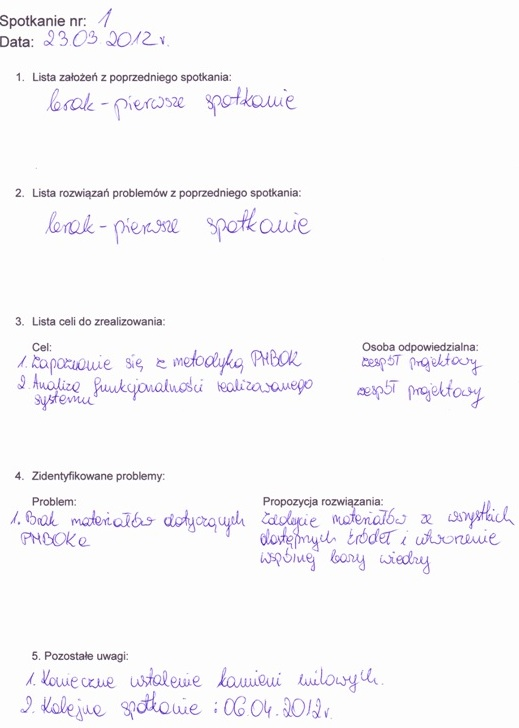
\includegraphics[width=.95\textwidth]{notatka.jpg}
\caption{Notatka z pierwszego spotkania wg. zdefiniowanego szablonu}
\label{fig:notatka}
\end{figure}
